\chapter{Applications of \acs{HPG-GdF}: Assessing vascular normalization using an antiangiogenic chemotherapy}
\label{ch:HPG3}

Through various signalling pathways, cancerous cells within tumours co-opt host vessels to obtain nutrients for rapid growth and creation of new blood vessels (angiogenesis)~\cite{Jain:2005gk}.
As the tumour expands a new vascular network is formed but is structuraly and functionally abnormal on account of leaky and tortuous blood vessels~\cite{McDonald:2002ut}, absent or loosely attached pericytes that provide structural support for cells, and abnormal morphology of the endothelial cells lining the vessels. 
Aberrant angiogenesis, poor blood perfusion, and a chaotic vascular network all play a role to limit oxygen delivery to cells, contribute to acidosis and formation of hypoxic regions in tumours~\cite{Jain:2005gk}.
Hypoxic regions within tumours are extremely problematic as those cells are resistant to both radiation and many cytotoxic chemotherapies.
Additionally, the resulting tumour microenvironment poses strong barriers to effective drug delivery and consequently, efficacy. 

A strategy to mitigate such adverse conditions of drug delivery is to attempt to normalize the vascular network by pruning away newly formed vessels, limiting creation of new vessels, and ultimately, spreading out the same amount of nutrients over fewer vessels.
As the structural components of the vasculature improve through reduced vessel leakiness and increased network organization, delivery of chemotherapies is more efficient~\cite{Jain:2001uf}.
This effect has been termed `Vascular Normalization` and does not just rely upon increased uptake of drugs and oxygen but also on improving the delivery of the drugs to a larger population of the tumour~\cite{Jain:2005gk}.
Considerable evidence has been presented in the literature in support of the vascular normalization window~\cite{Jain:2005gk,Viallard:2017ck,Martin:2019io}.
Several MRI techniques such as \acs{DCE-MRI}, \acs{DSC-MRI}, and \acs{ASL} have been used to obtain surrogate parameters of the effects of vascular normalization including cerebral blood volume and flow (CBV, CBF), \acs{K$^{trans}$}, \acs{$v_e$}, and \acs{$v_p$} ~\todo{add a couple of refs here, check Gerstner 2008}.
\acs{DCE-MRI} vessel permeability is typically measured using \acs{K$^{trans}$}, the volume transfer constant and is dependent on both vascular permeability and capillary surface area (related to blood flow) ~\cite{Tofts:1999we}. 
Unfortunately, because permeability and flow are highly coupled in the measurement \acs{$K^{trans}$}, interpretation of this parameter varies depending on the \emph{in-vivo} situation~\cite{Gerstner:2008ba}.
For instance, in regions of high permeability, the movement of the contrast agent is limited by blood flow so \acs{K$^{trans}$} primarily measures blood flow.
When applied in regimes of low permeability, the small molecular weight contrast agent cannot extravasate from vessels so \acs{K$^{trans}$} primarily measures vessel permeability~\cite{Tofts:1999we}.
These limitations motivated this work to determine whether a high molecular weight agent such as \acs{HPG-GdF} could be used for measuring vessel permeability without the confounding effects of blood flow.

The binding of \acs{VEGF} vascular endothelial growth factors (VEGF) to the VEGF receptor is a key driver of angiogenesis.
Bevacizumab - marketed clinically under `Avastin` - is a monoclonal antibody that binds VEGF extracellularly, preventing the interaction of of VEGF to its receptors and inhibits angiogenesis. 
Amongst others, Bevacizumab has been used clinically to treat breast, colon, colorectal, lung, brain, ovarian and cervical cancers~\cite{Genentech:2019th}. 
VEGF ablation has been shown to at least temporarily reduce vascular permeability and increase tumour oxygenation in some models~\cite{OConnor:2012ie}.
We hypothesized that after treatment with a \acs{VEGF} inhibitor will result in a decrease of vessel permeability as measured with \acs{DCE-MRI} with HPG-GdF.


\section{Methods}
\subsection{Mice tumours, and treatment groups}

All animal experimental procedures were carried out in compliance with the guidelines of the Canadian Council for Animal Care and were approved by the institutional Animal Care Committee. 
Twelve female NOD-SCID mice were implanted with murine squamous cell carcinoma SCCVII tumours (5 x 10$^5 $cells in 50 $\mu$l serum-free media; cells provided by Dr. J Evans).
Mice were imaged when the largest tumour diameters reached a volume of approximately 500 mm$^3$, positioned supine on the custom surface coil apparatus and anesthetized with isoflurane for the duration of imaging sessions until euthanasia.

The treated group comprised six of the twelve animals and were administered 5mg/kg mouse anti-VEGF antibody (B20-4.1.1., Genentech) 72 hours prior to the imaging session.
Throughout the imaging session, a small animal monitoring system (SAII Instruments, Stony Brook, NY, USA) was used to monitor respiration rate and body temperature. 
A continuous airflow heater was used to maintain temperature at 36.5 $\pm$ 1$^\circ$C.
All animals were injected with 60 mg/kg pimonidazole hydrochloride (HypoxyProbe) intraperitoneally 60 minutes prior to imaging to label hypoxic cells and were euthanized within 15 min of imaging completion.
Tumours were embedded and frozen in optimum cutting temperature medium (OCT; Tissue-TEK).
%Carbocyanine was injected intravenously through the tail vein 5 minutes prior to euthanasia.

\subsection{MRI}
MRI experiments were performed at the UBC MRI Research Centre on a 7T Bruker Biospec 70/30 scanner at room temperature with a combination volume (transmit)/surface (receive) coil.
DCE-MR imaging data was collected as previously described [19].~\todo{bring in relevant details for thesis}
Macromolecular contrast agent hyperbranched polyglycerol \acs{HPG-GdF}, 500 kDa) was synthesized as previously described [20, 21] and administered as a 6 $\mu$L/g bolus dose from 100 mg/mL (0.2 mM).
Regions of interest (ROI) were drawn on T2-weighted RARE images to outline the tumour using ImageJ (NIH) and all other MR analysis was performed using Python.
A two-parameter linear model was applied to characterize \acs{HPG-GdF} signal-intensity curves for \acs{fPV} determined by the rapid increase at time of injection and for \acs{aPS} calculated as the slope of later enhancement.
Area Under the Curve (\acs{AUC}) for \acs{HPG-GdF} was determined using the signal intensity curves from the injection time point to 60s.
Non-enhancing voxels (i.e. those with an AUC$_{60} < 0$) were excluded from all analyses.
Both MR and histological modalities imaged slices in the plane perpendicular to an implanted fiducial marker tube to minimize angular differences between MR and histological image slices~\cite{Bains:2009hh}.

\subsection{Immunohistochemistry}
%The general immunohistochemical procedure used has been previously reported [16].
Frozen and OCT-embedded tumours were cryosectioned into 10$\mu$m thick slices and air-dried.
Sections were first imaged for native DiOC7(3) or Alexa 647nm-tagged \acs{HPG-GdF} fluorescence, and fixed in 50\% (v/v) acetone/methanol for 10 minutes at room temperature.
Additional staining was performed using antibodies to PECAM/CD31 (BD PharMingen) and pimonidazole (hypoxprobe).
Visualization of primary detection antibodies was done using Alexa fluorescence secondary antibodies of appropriate species using 488 nm and 546 nm wavelengths.
Nuclear density was stained using Hoechst 33342 (Thermofisher) and imaged at 380 nm.

\subsection{Image acquisition and analysis}
Sections were imaged using a system of tiling adjacent microscope fields of view at a resolution of 0.75 $\mu$m/pixel~\cite{Kyle:2007ch}.
Using ImageJ~\cite{Collins:2007jr} and user-supplied algorithms, images were superimposed and manually cropped to tumour tissue boundaries with staining artifacts and necrosis removed.
False color images were constructed in ImageJ by converting greyscale images to color and overlaying selected layers: \acs{HPG-GdF} (red), Hoechst 33342 (grey), CD31 (blue), carbocyanine (cyan), pimonidazole (green).
Positive fluorescent staining for each slice is reported as a mean, and the median group intensity $I$ (range 0-255) is reported for pimonidazole ($I_{pimo}$), \acs{HPG-GdF} ($I_{hpg}$) and CD31 ($I_{CD31}$)~\todo{remove CD31 if not showing in results}.

\section{Results}

\subsection{Treatment with B20 reduces tumour hypoxia 72 hours after treatment}

Treatment with the \acs{VEGF} inhibiting drug B20 resulted in a dramatic reduction in hypoxia in SCCVII tumour xenografts.
Immunohistological staining with pimonidazole allowed for visualization of these group differences with a representative example shown in figure~\ref{hpgB20:histohpgpimo}.
In the untreated group, large regions of the tumours are hypoxic though there is considerable heterogeneity in baseline hypoxia status between tumours and between slices of the same tumour.
In the treated group, pimonidazole staining is disparate and not concentrated in local regions of poor oxygenation.
Treated tumours also had relatively lower levels of bound pimonidazole and this was consistent across tumours and between slices of the same tumour.
These staining patterns are representative, but there is considerably more heterogeneity in pimonidazole staining in the control tumours.

\begin{figure}[htbp] % figure placement: here, top, bottom, or page
  \centering
  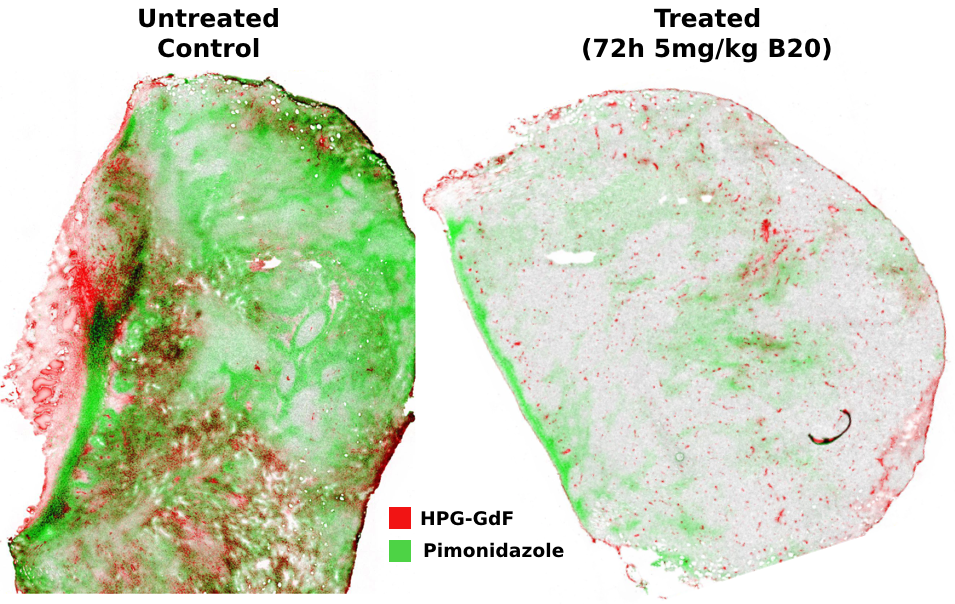
\includegraphics[width=0.8\textwidth]{hpg/hpg-B20-images/histo_hpgPimo.png} 
  \captionsetup{width=\linewidth}
  \caption{Histological sections of a control (left) and treated tumour (right) are shown to illustrate the dramatic decreases both in pimonidazole staining and in accumulation of \acs{HPG-GdF} in the treatment group.}
  \label{hpgB20:histohpgpimo}
\end{figure}

Quantitative analysis of the immunohistolgoical stains in the images was conducted to assess whether these observations existed at the group level. 
A Mann-WhitneyU test indicated that the median pimonidazole staining intensity was greater for the control group ($I_{pimo}$ = 21.7) than the treated group ($I_{pimo}$ = 17.2), $U = 47$, $p = 5\times10^{-5}$.
Group difference plots are shown in figure~\ref{hpgB20:accumulation}.

\begin{figure}[htbp] % figure placement: here, top, bottom, or page
  \centering
  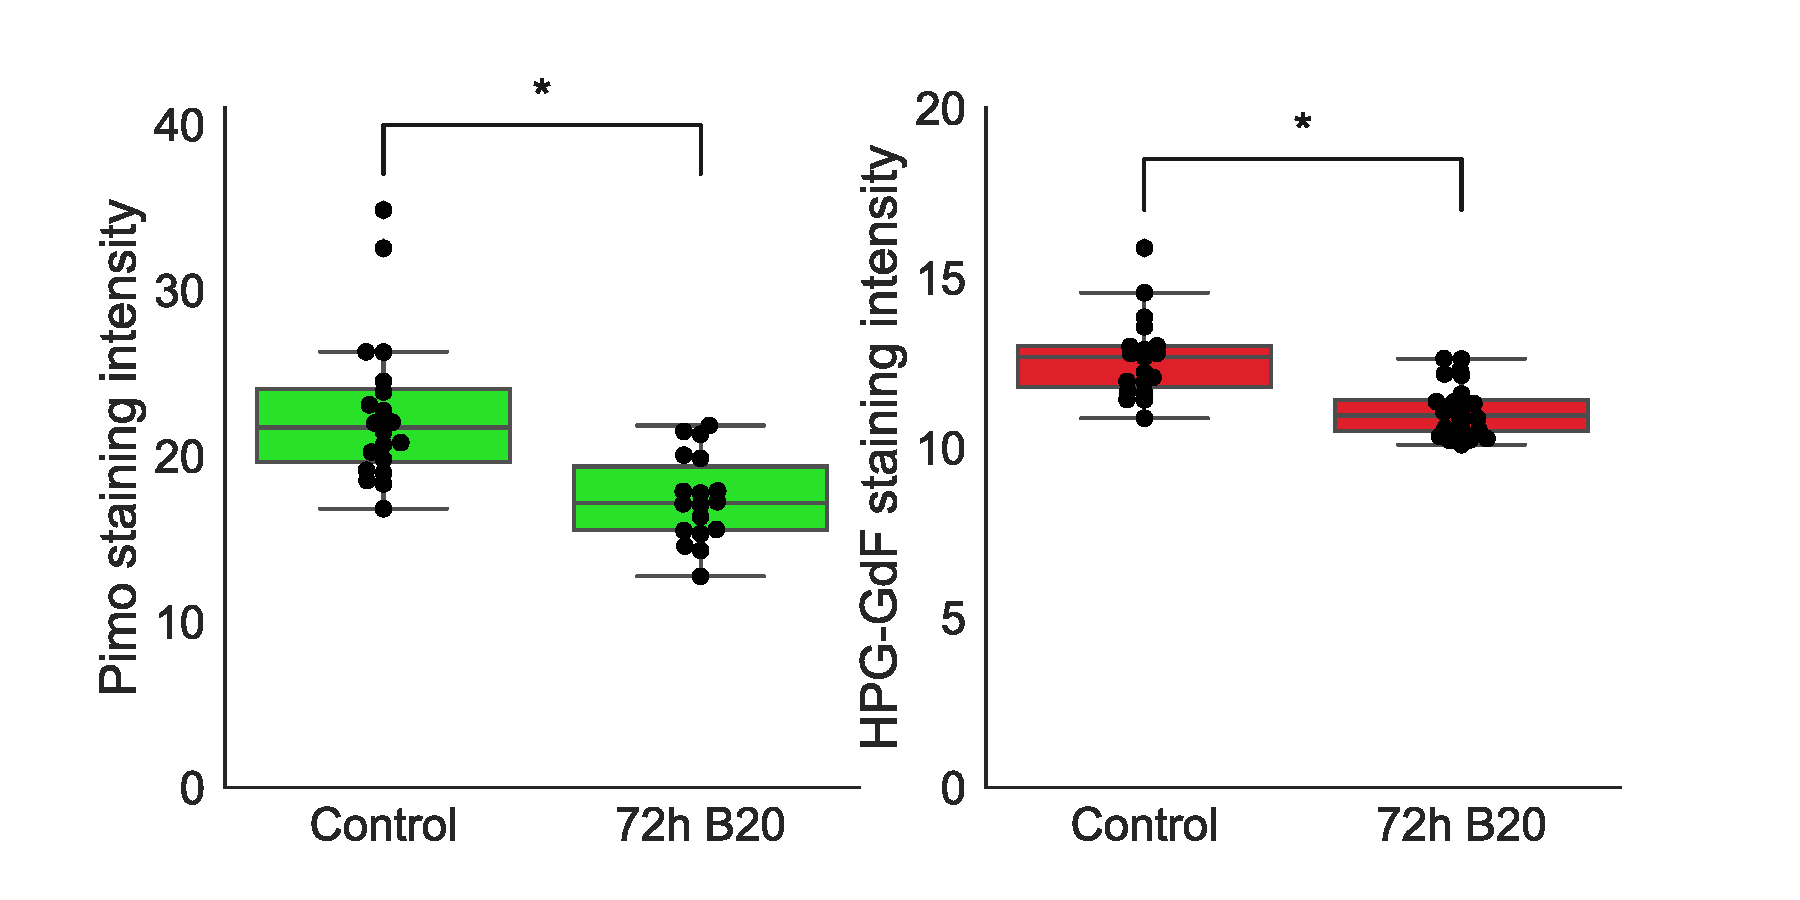
\includegraphics[width=0.8\textwidth]{hpg/hpg-B20-images/hpg_pimoHPG-GdF.pdf}
  %\captionsetup{width=\linewidth}
  \caption{Median pimonidazole staining is markedly reduced for the B20-treated group ($I_{pimo} = 17.2$) compared to the controls ($I_{pimo} = 21.7$).
  Median \acs{HPG-GdF} staining intensity is also reduced for the treated tumours ($I_{hpg} = 12.7$) compared to the controls ($I_{hpg} =11.0$).
  P-values from the Mann-WhitneyU test were $p = 5\times10^{-5}$ (pimo, left) and $p = 8\times10^{-6}$ (\acs{HPG-GdF} fluorescence, right).}
  \label{hpgB20:accumulation}
\end{figure}

\subsection{Blood vessel permeability (\acs{aPS}) and HPG-GdF accumulation (fluorescence intensity) decreases in tumours treated with B20}

Apparent permeability-surface area product (\acs{aPS}) is a parameter that captures vessel leakiness with \acs{DCE-MRI} using the large molecular weight contrast agent~\acs{HPG-GdF}.
Figure~\ref{hpgB20:accumulation} shows the group differences and the median value of the B20-treated group (aPS$_{Md}$ = $1\times10^{-4}$) was significantly lower than the control group (aPS$_{Md}$ = $6.5\times10^{-5}$); Mann-Whitney $U = 3$, $p = 0.01$.

Histological staining of \acs{HPG-GdF} fluorescence matched relatively well with areas of high \acs{aPS} values as shown in figure~\ref{hpgB20:aPSaccumulation}, however there are also areas where aPS is moderate to high but \acs{HPG-GdF} fluorescence is not present in high concentrations. 
Differences in \acs{HPG-GdF} accumulation were also present histologically as \acs{HPG-GdF} fluorescence intensity was markedly decreased in the B20-treated group ($I_{hpg} = 12.7$) compared to the controls ($I_{hpg} = 11.0$); a Mann-WhitneyU test indicated the difference was significant $U = 52$, $p = 9\times10^{-6}$.
Aggregate voxel distributions of \acs{aPS} values in Figure~\ref{hpgB20:accumulation} also shows a clear reduction in \acs{aPS} in the treatment group.Figure~\ref{hpg:aPShistoEC} shows the \acs{aPS} parametric maps from \acs{DCE-MRI} alongisde approximate slice matched histology sections from the same tumours.
Patterns observed in the quantitative analysis of the data are also evident in MRI and histology images: following treatment with B20, there is a marked reduction in blood vessel permeability measured by \acs{aPS} and a reduction in \acs{HPG-GdF} accumulation histologically measured by native fluorescence of the contrast agent.

\subsection{\acs{HPG-GdF} enhancement curves and \acs{AUC}$_{60}$ are altered after treatment, but \acs{fPV} does not change}

Group \acs{HPG-GdF} enhancement curves are shown in Figure~\ref{hpg:aPShistoEC} and match the results obtained from a quantitative analysis of the parameteric maps: treated tumours have a relatively flat profile and plateau whereas the control tumours show a steady increase of enhancement arising from the leakage of \acs{HPG-GdF}.
\acs{AUC}$_{60}$ is a parameter that captures the relative enhancement of voxels within the first 60 seconds after injection.
The control tumours had a median \acs{AUC}$_{60-Md} = 5.5$ and treated tumours had a median \acs{AUC}$_{60-Md} = 4.0$ and the reduction was statistically significant (Mann-Whitney $U = 6, p = 0.03$).
The \acs{fPV} values for the control (fPV$_{Md} = 0.12$) and treated tumours (fPV$_{Md} = 0.09$) were not significantly different (Mann-Whitney $U = 3, p = 0.15$).

\begin{figure}[htbp] % figure placement: here, top, bottom, or page
  \centering
  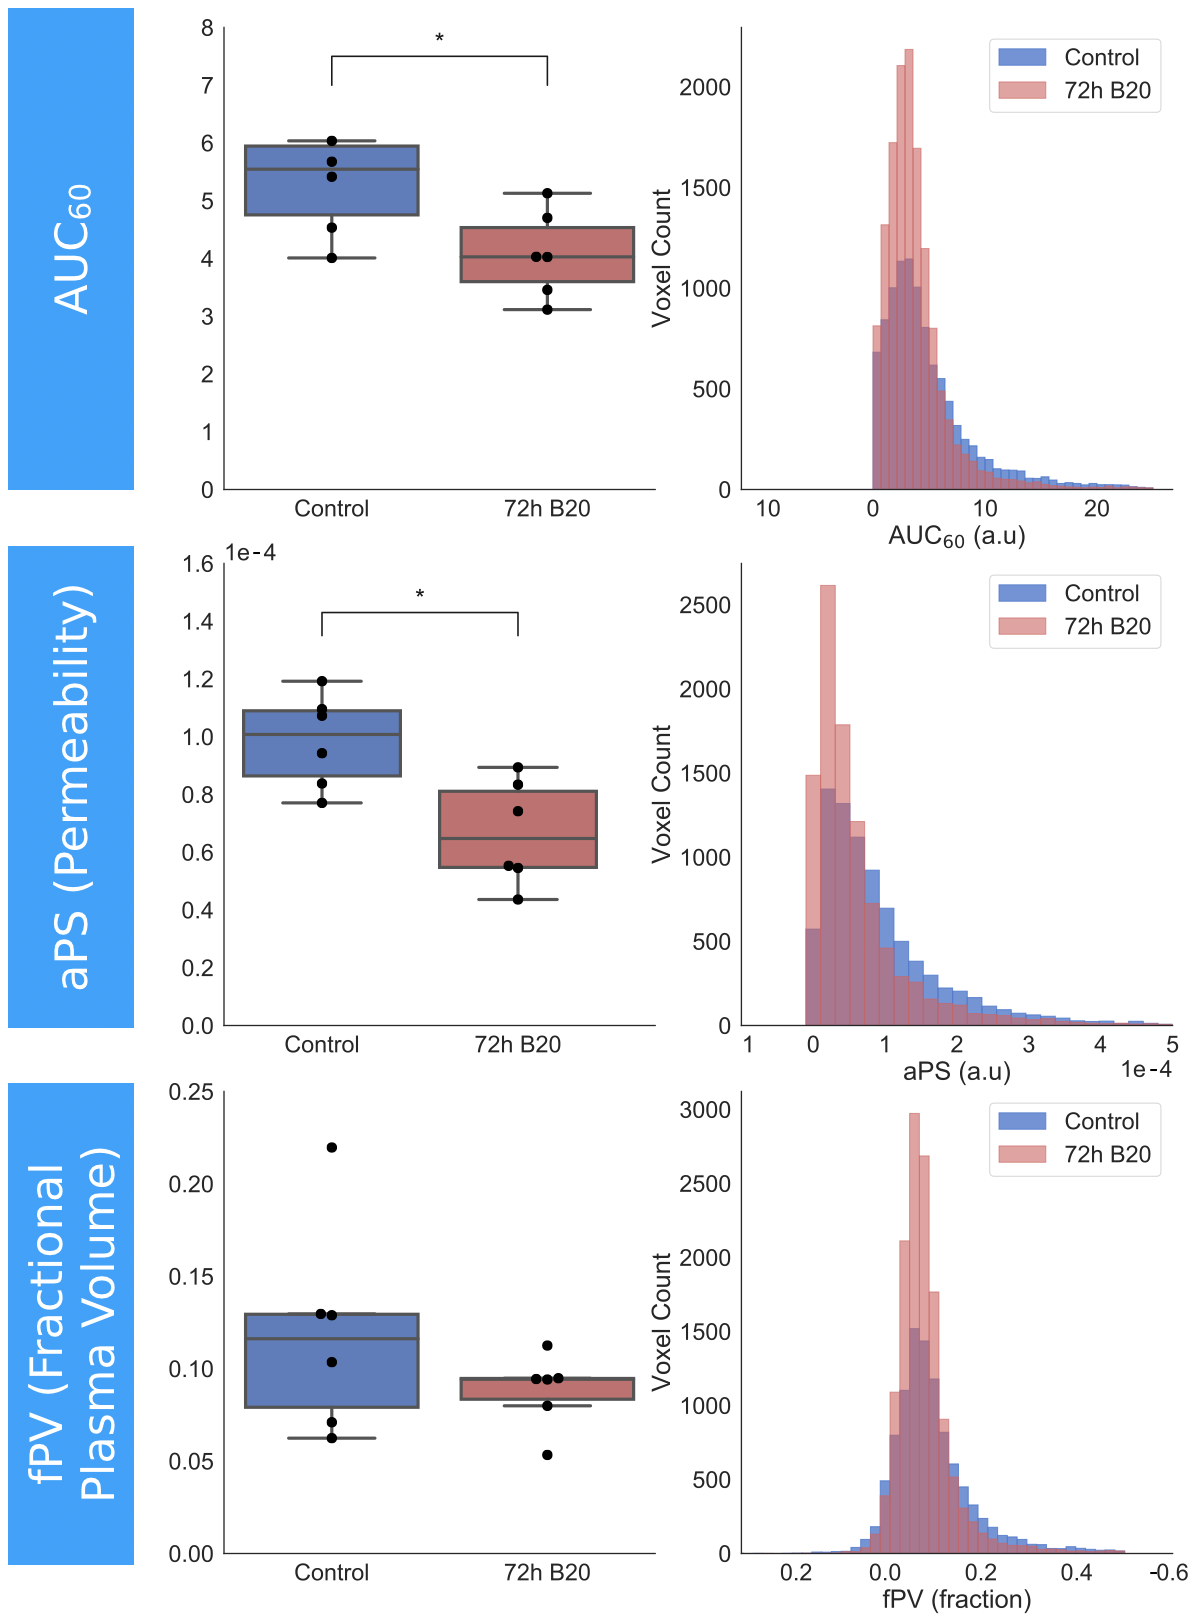
\includegraphics[width=0.8\textwidth]{hpg/hpg-B20-images/hpg_mriparams.png} 
  %\captionsetup{width=\linewidth}
  \caption{Summary of group differences for all three \acs{DCE-MRI} parameters: \acs{AUC}$_{60}$, \acs{aPS}, and \acs{fPV}. 
  There is a statistically significant reduction in \acs{AUC}$_{60}$ and \acs{aPS} for the treated tumours, but no difference measured for \acs{fPV}.
  P-values from the Mann-WhitneyU statistical test for the comparisons were $p=0.03$ (\acs{AUC}$_{60}$), $p=0.01$ (\acs{aPS}), and $p=0.15$ (\acs{fPV}).}
  \label{hpgB20:aPSaccumulation}
\end{figure}

\begin{figure}[htbp] % figure placement: here, top, bottom, or page
  \centering
  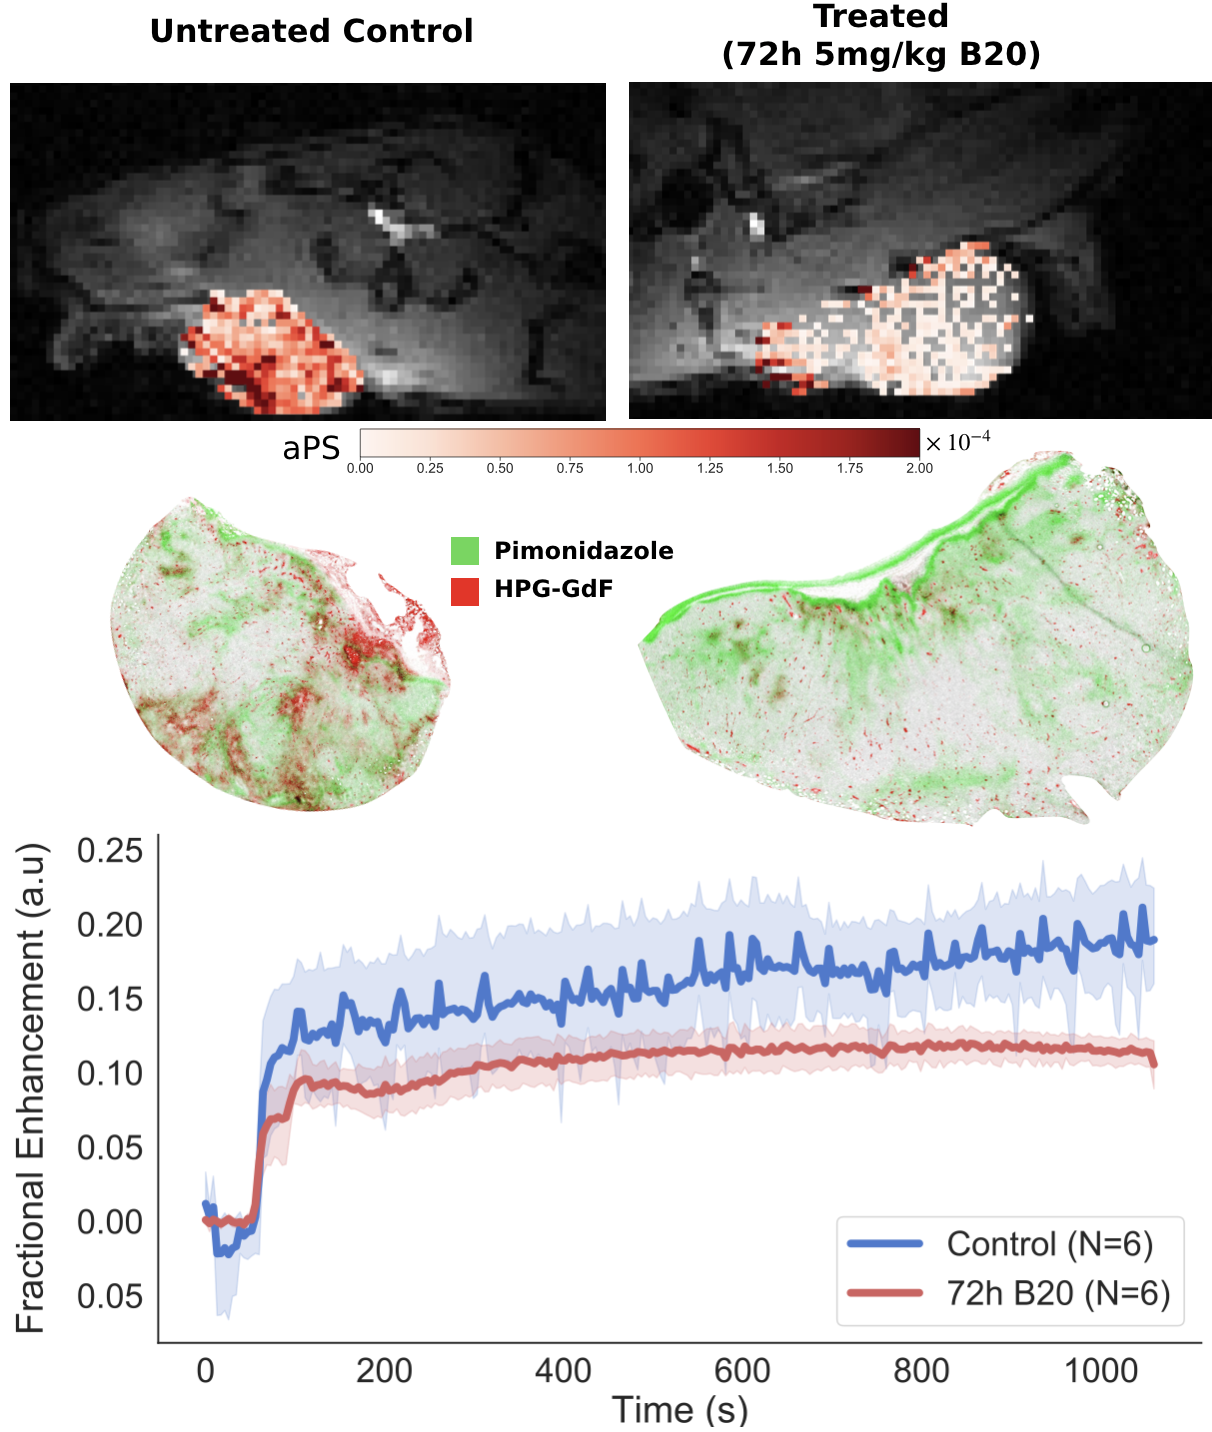
\includegraphics[width=0.8\textwidth]{hpg/hpg-B20-images/hpg_aPShisto_ec.png} 
  \captionsetup{width=\linewidth}
  \caption{Histological stains of \acs{HPG-GdF} shown alongside approximate slice matched \acs{DCE-MRI} parameter map of \acs{aPS} and the group-averaged contrast enhancement curves of control and treated tumours. There is an overall reduction in \acs{aPS} for the treated tumours. The mean contrast enhancement curves (group means in dark blue and red lines; shaded region is the 95\% confidence interval determined by bootstrapping) also show that the treated tumours have a higher enhancement slope after contrast agent injection.}
  \label{hpg:aPShistoEC}
\end{figure}

% Need full data to say this, can put images in an appendix?
%- Low inter-tumour slice variability in average staining intensity of \acs{HPG-GdF} fluorescence 
%- Heterogeneity in tumour response, not all tumours responded consistently

\section{Discussion}

In this study we have demonstrated that \acs{DCE-MRI} with \acs{HPG-GdF} is useful for assessing vessel permeability using the apparent permeability-surface area product, \acs{aPS}.
This application is further validation of the utility of the high molecular weight agent \acs{HPG-GdF} in exploring the tumour microenvironment.
Comparing direct \acs{HPG-GdF} fluorescence on cryosections with \acs{DCE-MRI} parameters \acs{aPS} and \acs{fPV}.

- sccvii tumours have almost no necrosis, which makes this a useful model contrast agent accumulation. Otherwise agent pools into empty space and is difficult to quantiy or assess

- there was some heterogeneity in HPG staining within tumour slices, and even between tumours but on aggregate it is clear that the treated tumours had significantly less HPG accumulation

- aPS parameter corresponds to permeability; rate of enhancement change over time, this trend is also observed in the enhancement curves

- As shown in Figure~\ref{hpg:aPShistoEC}, there is considerably less variability in the enhancement curves of the treated tumours, strong evidence for B20 normalizing the vasculature.

- auc60 of the intensity, which represents presence of HPG in the blood 60s after injection was also sig different --> more evidence that the treatment altered the tumour vasculature

- pimo decrease was quite stark

- Increased oxygenation could not be assessed with existing MRI techniques so this result was only observed with immunohistochemistry.

- unclear why there is hpg staining in regions that are clearly hypoxic. intermittent hypoxia as a potential explanation?

- We should look for non-invasive imaging based methods to deal with this.

-- limitations
- signal intensity vs. contrast agent concentration (requires AIF, complicated modeling, not clear if that approach is superior to IAUC but validation with histology is a positive sign that this approach is valid)
- no way to measure oxygenation change in vivo, would be nice to confirm that lower pimo staining also means lower oxygenation levels in the tumour
- worth doing a larger study with more sections in the tumour to explore intertumour heterogeneity, accounting for tumour size and treatment effect

\section{Conclusion}

- aPS decreases after administration of B20, confirmed by histology direct hpg fluorescence imaging; vessels are less leaky after treatment
- less auc60 for treated mice also indicates less hpg accumulation histologically in treated compared to controls
- HPG-GdF was used to demonstrate that the vasculature became more normal
\endinput